\documentclass[UTF8]{ctexart}
\usepackage{mathtools,wallpaper}
\usepackage{t1enc}
\usepackage{pagecolor}
\usepackage{enumitem}
\usepackage{hyperref}
\usepackage{graphicx}
\usepackage{listings}
\usepackage{amssymb}
\usepackage[dvipsnames]{xcolor}
\usepackage{float}
\usepackage{numerica}


\begin{document}

\section{Turing Machine}
\subsection{The basic case of Turing Machine}

\begin{itemize}
    \item The components of TM
    \begin{enumerate}
        \item An infinite tape
        \item A finite-state control unit(state set)
        \item A single head which reads symbols from the tape and changes symbols on the tape.
    \end{enumerate}
    \item The property of tape
    \begin{enumerate}
        \item tape有一个左端点，右端可以无限延伸。为了防止将指针头移除左端，tape的最左端点加了一个$\rhd $,一旦指针头读到$\rhd $，我们就立马将指针左移动一位。
        \item 我们使用$L$和$R$表示指针头向左移动或者向右移动
        \item 纸带上空用$\sqcup $表示。
    \end{enumerate}
    \item The definition of TM
    \begin{figure}[H]
        \centering
        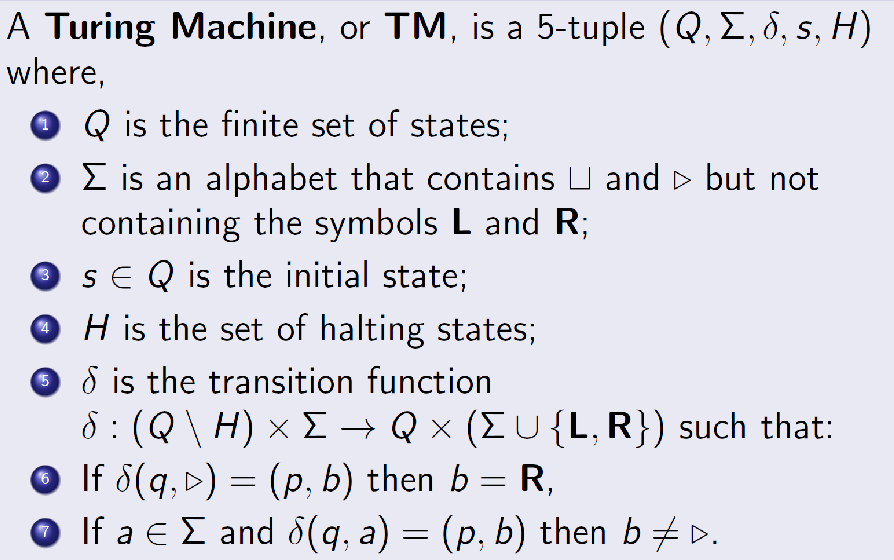
\includegraphics[width=1\textwidth]{static/Component-of-TM.png}
        \caption{Component-of-TM}
        \label{Component-of-TM}
    \end{figure}
    \begin{enumerate}
        \item Q是有限状态集合
        \item $\sum$是包含$\sqcup $和$\rhd $但是不包含\textbf{L}和\textbf{R}的字母表
        \item $s \in Q$是初始状态
        \item $H$ 是终止状态集合
        \item $\delta$ 是转移方程，左边是 非停机状态*字母表 的输入组合，右边是新状态*(要写符号以及移动方向)的组合
    \end{enumerate}

    以下是七元组的图灵机：
    \begin{figure}[H]
        \centering
        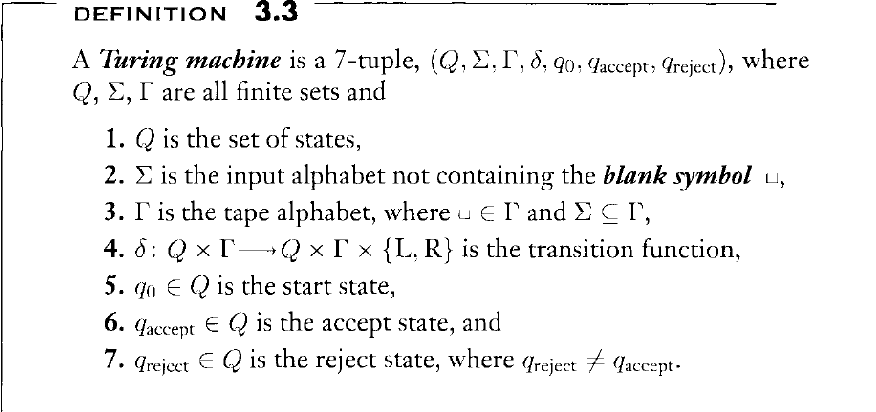
\includegraphics[width=1\textwidth]{static/Tuple7ML.png}
        \caption{Tuple7ML}
        \label{Tuple7ML}
    \end{figure}

\end{itemize}

\subsection{Configuration}
\begin{itemize}
    \item 为了清晰地看清当前图灵机的Configuration，我们将纸带分为两个部分，左边部分包括从指针头指到的扫描格到最左边，右边部分是不包括当前扫描到的鸽子的扫描格右边的部分。
    \item Configuration of TM
    \begin{figure}[H]
        \centering
        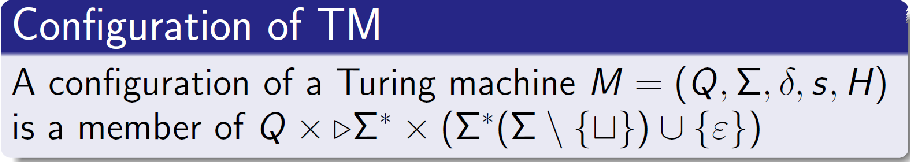
\includegraphics[width=0.7\textwidth]{static/Configuration-of-ML.png}
        \caption{Configuration-of-ML}
        \label{Configuration-of-ML}
    \end{figure}
     TM的配置，第一个是状态，第二个是以$\rhd$开头的由字母表中的符号组合成的字符串，第三个部分前面就是扫描到的表格的右边部分的字符串集合+不能以$\sqcup $结尾，结尾要以$\epsilon$结尾。
    \begin{figure}[H]
        \centering
        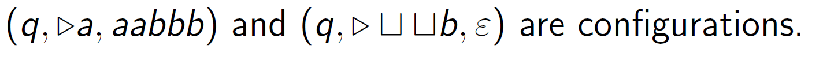
\includegraphics[width=0.7\textwidth]{static/Configuration-eg.png}
        \caption{Configuration-eg}
        \label{Configuration-eg}
    \end{figure}
    \begin{figure}[H]
        \centering
        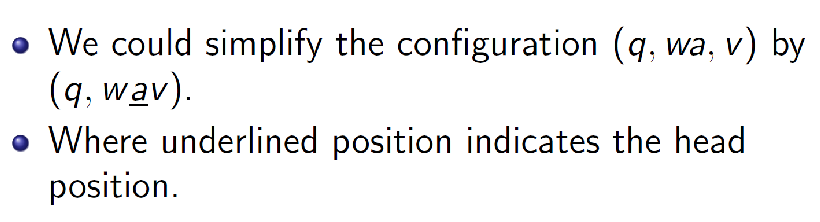
\includegraphics[width=0.7\textwidth]{static/Simplify-Configuration.png}
        \caption{Simplify-Configuration}
        \label{Simplify-Configuration}
    \end{figure}

\end{itemize}

\subsection{Computation}

    \begin{figure}[H]
        \centering
        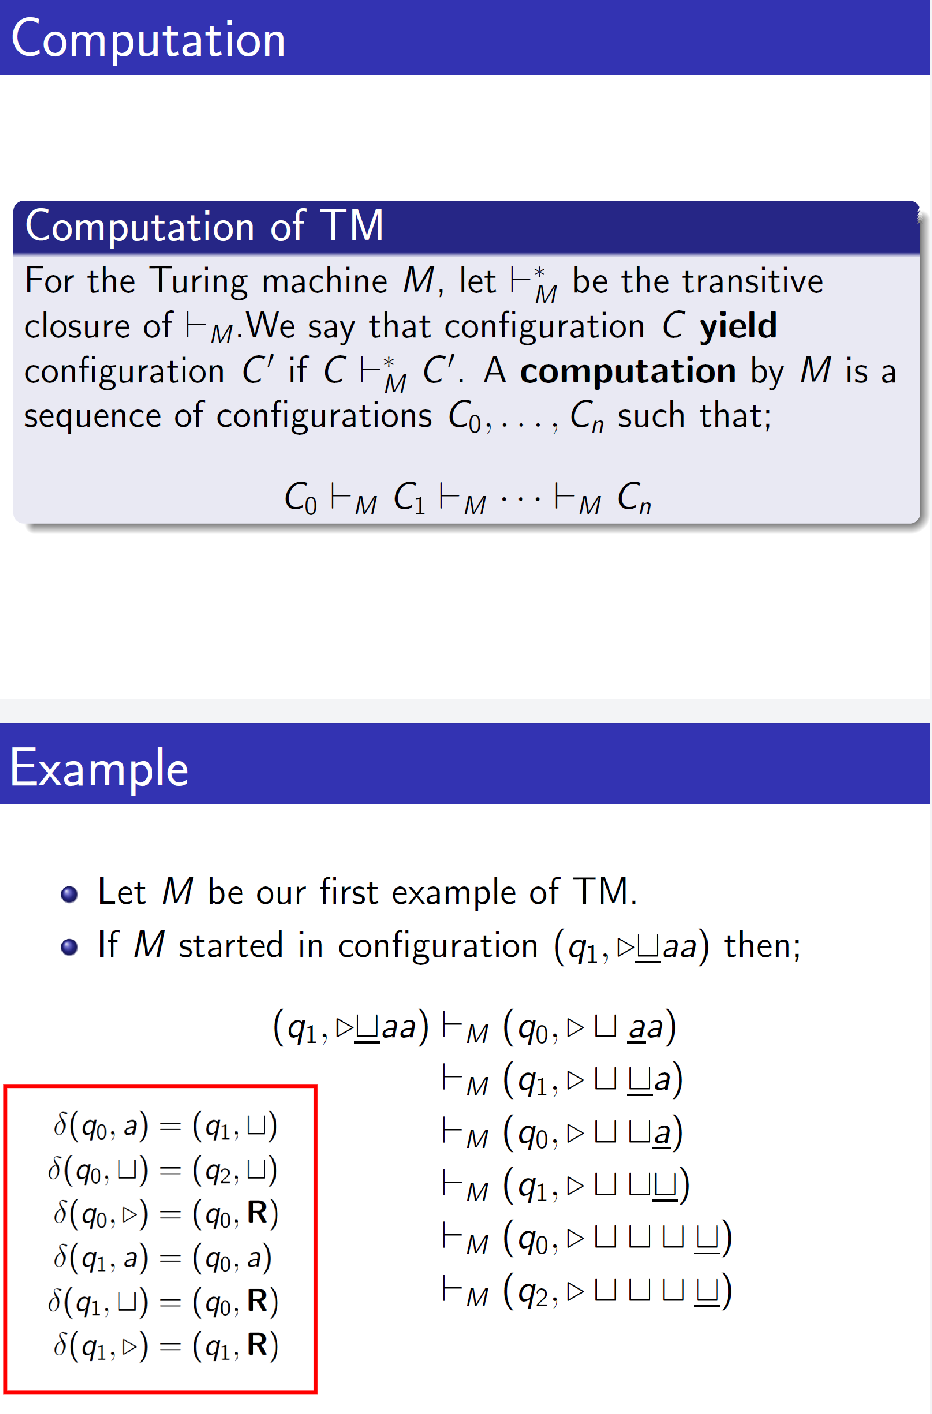
\includegraphics[width=0.7\textwidth]{static/Computation.png}
        \caption{Computation}
        \label{Computation}
    \end{figure}

\subsection{Symbol Writing and Head-Moving}
\begin{itemize}
    \item eg1
    
    对于每一个a属于字符集并上L，R但是不包括$\rhd $.我们定义一个图灵机$M_a$,状态集合包含start和halt两个状态，字符表，状态转移方程，开始状态，结束状态。对于每一个b属于字母集但是不包含$\rhd$，状态转移方程如果状态是s，当前字母是b中的一个字母，那么变为halt状态，当前字母修改为a中的某一个字母。如果当前状态是s，当前字母是$\rhd$，那么图灵机自动从开始状态向右移动一位。所以如果a属于字母集合中，那么图灵机就会写下一个a，并且叫此图灵机为符号书写机，如果a是L和R字母中的一个，我们就向左或者向右移动，并且称之为head-moving machine。

\end{itemize}

\subsection{Combining Machines}
\begin{itemize}
    \item 如果$M_1$和$M_2$是图灵机，那么我们可以将两个图灵机组成一个新的图灵机。
    \item 从$M_1$到$M_2$，只有当$M_1$停止之后，$M_2$从$M_1$停止的状态和head的位置作为初始状态和head的位置。
    \item eg2
    \begin{figure}[H]
        \centering
        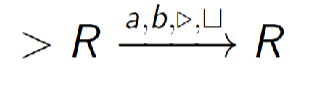
\includegraphics[width=0.7\textwidth]{static/SimpTMeg1.png}
        \caption{SimpTMeg1}
        \label{SimpTMeg1}
    \end{figure}
    这张图表示首先将head先向右移动一个square，如果此square是a，b，右箭头和blank，则再向右移动一个箭头。如果箭头上的字母是字母表中的所有字母，则可以将字母省略，只写一个箭头。再进行简化，将箭头去掉RR。最后简化为$R^2$，means that 先将head向右移动2次。
\end{itemize}

\subsection{Simple Turing Machines}
\begin{itemize}
    \item eg1
    
    以下TM表示图灵机将会一直向右进行扫描，直到遇到blank，可以用$R_\sqcup $表示。
    \begin{figure}[H]
        \centering
        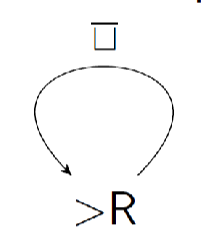
\includegraphics[width=0.3\textwidth]{static/SimpTM1.png}
        \caption{SimpTM1}
        \label{SimpTM1}
    \end{figure}

    \item eg2
    
    以下TM表示图灵机将会一直向左进行扫描，直到遇到blank，可以用$L_\sqcup $表示。
    \begin{figure}[H]
        \centering
        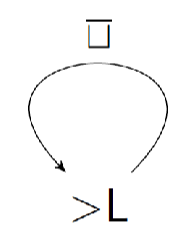
\includegraphics[width=0.3\textwidth]{static/SimpTM2.png}
        \caption{SimpTM2}
        \label{SimpTM2}
    \end{figure}

    \item eg3
    
    以下TM表示图灵机将会一直向右进行扫描，直到遇到non-blank，可以用$R_{\overline{\sqcup}}$表示。
    \begin{figure}[H]
        \centering
        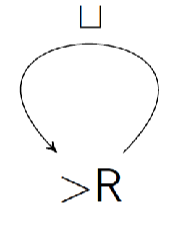
\includegraphics[width=0.3\textwidth]{static/SimpTM3.png}
        \caption{SimpTM3}
        \label{SimpTM3}
    \end{figure}

    \item eg4
    
    以下TM表示图灵机将会一直向左进行扫描，直到遇到non-blank，可以用$L_{\overline{\sqcup}}$表示。
    \begin{figure}[H]
        \centering
        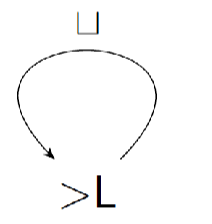
\includegraphics[width=0.3\textwidth]{static/SimpTM4.png}
        \caption{SimpTM4}
        \label{SimpTM4}
    \end{figure}
\end{itemize}

\subsection{Computing With Turing Machine(recognize language)}

\begin{itemize}
    \item 如果一个五元组的图灵机器M=($Q,\Sigma ,\delta ,s,H$),H=\{y,n\}。停机状态中的y被称为accept configuration,停机状态中的n被称为rejecting configuration。
    \item 让字符集$\Sigma_0=\Sigma \setminus \{\sqcup ,\rhd \}$，图灵机M能够decides一个语言$L\subseteq \Sigma_0^{*}$如果对于任意字符串$\Sigma_0^{*}$我们有：如果输入$w \in L$，那么M停机输出accept；如果$w \notin L$,M停机输出reject。
    \item Recursive Language(递归语言)
    \begin{enumerate}
        \item 一个语言是递归语言，如果有一个图灵机能够判定这个语言。
        \item 称一个语言是图灵可判定的(turing-decidable),如果某些图灵机可以判定此语言。
        \item 如果L是一个recursive language 那么L的补也是可递归的。
    \end{enumerate}
    \item Function by TM
    
    定义：M是五元组图灵机，字符集$\Sigma_0=\Sigma \setminus \{\sqcup ,\rhd \}$是输入，并且w是字符集中组成的某个字符串。假设M在输入w停机，并且(s,$\rhd \underline{\sqcup} w$)$\vdash_M^{*}$$(h,\rhd \underline{\sqcup} y)$并且$y \in \Sigma_{0}^{*}$,那么y被称为M在输入w都输出(记作M(w))。
    \item Recursive Function
    
    定义：让f是从除了空和右三角号的字符集组成的某个字符串到某个字符串的映射。称M计算f，对于所有w属于字符串的子集，M(w)=f(w)。并且f(w)能够被定义仅当M在w上停机。我们称函数f是recursive。
    
    \item Multivariable Functions 计算多元自然数函数
    
    定义：M是一台五元组图灵机，字符集包括0，1，；。并且让函数f从k个自然数作为输入映射为单个自然数作为输出。我们称M计算函数f如果对于所有的从w1到wk属于至少含有一个0或者1的输入，num(M(w1;...;wk))=f(num(w1),...,num(wk)).我们称此方程f是递归的。

    \item Recursively Enumerable递归可枚举
    
    定义：M是五元组的图灵机，并且L是含于不包括空格和空的字符集组成的字符串子集中的一个语言。我们称M是 semidecides L如果对于任何字符串w属于字符串子集我们有：w属于L当且仅当M在w上停机。一个语言是recursively enumerable/turing recognizable 当且仅当有一个图灵机能够semidecide这个语言。
    \begin{enumerate}
        \item 如果w属于不包括空格和空的字符集组成的字符串子集，但是不属于L，并且L是递归可枚举，那么w将不会到达停机状态。
        \item So M semidecide L if for any string \(w \in \sum _{0}^{*}\) we have; \(M(w)=\nearrow\) if and only if w e L
    \end{enumerate}

    \item recursive vs recursively enumerable
    \begin{enumerate}
        \item 定理：每一个递归语言都是递归可枚举的。
        
        证明：假设M是一个五元组图灵机并且停机状态包含n(reject)。有一个M‘是一个停机状态不包含n的五元组并且转换方程中的(n,a)变为(q,a)，那么状态n在M‘中不是一个停机状态，而是一个循环。所以如果M能够判定L，那么M’能够半判定L。所以判定含于半判定。

    \end{enumerate}

\subsection{Extensions of the turing machine}
\subsubsection{Multiple Tapes}

定义：一个k-tape五元组图灵机M，k大于等于1。转移方程输入部分为当前状态但是不能为停机状态，符号集为当前k条扫描符号的k元组映射到输出为下一状态，k条带到动作指令(包括字符集以及L，R)组成的k元组

\begin{itemize}
    \item Configuration of Multiple Tape TM
    
    定义：Let \(M=(Q, \sum , \delta, s, H)\) be a k-tape Turing machine. A configuration of M is a member of the following set: \[Q\times (\triangleright \sum ^{*}\times (\sum ^{*}(\sum \backslash \{ \sqcup \} )\cup \{ \varepsilon \} ))^{k}\]

    图灵机当前所处状态+第一部分从读写头开始到扫描符号的左侧（三角号+字符串集）+第二部分从读写头当前扫描符号开始到带右侧的所有符号，若带非空结尾不能为空白符，若带为空用空串符号表示。

    By \(\vdash_{M}^{*}\) we mean the transitive closure(转移关系闭包) of \(\vdash_{M}\)。\(\vdash_{M}\)表示一个configuration的转移，\(\vdash_{M}^{*}\)表示零次/一次/多次configuration的转移。

    \item 对于多带图灵机，每个动作指令的右上标表示让图灵机的第几个纸带做此操作。
    \item 每一个多带图灵机都于一个单带图灵机等价。
    
    证明：单带图灵机M必须以某种方式包含多带图灵机M‘当前状态下的所有信息。我们将单带图灵机的纸带划分为2k条轨道，奇数条轨道表示从1到k条纸带，偶数条轨道记录当前指针指在多带每一条带的哪一个位置，就在那个位置下赋值为1，其余赋值为0
    
\end{itemize}
\subsubsection{Two-way Infinite Tape}

\begin{itemize}
    \item 在基础图灵机的定义下，纸带是双向无限长的，并且没有右箭头，纸带从输入的左端开始。
    \item 定理：每一个双向无限纸带图灵机都可以等价为单纸带图灵机。
    
    证明：
    使用双带图灵机模拟双向无限纸袋图灵机，双带图灵机一条纸带表示从右到输入的纸带，第二条纸带以反向顺序存储指针头左侧的部分。
\end{itemize}

\subsubsection{Two-dimensional Tape}
每一步计算都有4种可能的操作Left,Right,Up,Down\{L,R,U,D\}。

每一个双维无限纸带图灵机都等价于一台单带图灵机。

\subsubsection{All Models Are Equivalent}
\begin{itemize}
    \item Every Nondeterministic Turing machine is equivalent with a deterministic Turing machine.
    \item Transition function of a Turing machine could be nondeterministic transition, i.e., 
\[\delta:(Q \backslash H) × \sum \to \mathcal{P}(Q \times(\sum \cup\{L, R\}))\],P是幂集。
or equivalently a subset of: 
\[((Q \backslash H) × \sum) \times(Q \times(\sum \cup\{L, R\}))\]
\end{itemize}
    
\end{itemize}

\subsection{Nondeterministic Turing Machine不确定性图灵机}

定义：非确定性图灵机是一个五元组(K,$\Sigma $, $\bigtriangleup $ ,s, H),K,$\Sigma $,s, H和标准图灵机相同，$\bigtriangleup $是集合\(((K-H)\times\sum)\times(K\times(\sum\cup\{L,R\}))\)的一个子集。

\begin{enumerate}
    \item 定义：M是一个五元组\(M=(K, \sum , \Delta, s,\{y, n\})\)的非确定性图灵机。M能够判定一个语言\(L \subseteq(\sum -{\triangleright, \sqcup})^{*}\)若以下条件满足\(w \in(\sum -{\triangleright, \sqcup})^{*}\)：

(1)存在一个自然数N(人为设定的最大执行步数)，对于给定的图灵机M和输入w，让机器从初始格局出发，连续执行N步转移后，无法到达任何合法格局。

(2)当且仅当\((s, \triangleright \underline{\sqcup} w) \vdash_{M}^{*}(y, u \underline{a} v)\),并且u \(v \in \sum ^{*}\) , \(a \in \sum\)，此时\(w \in L\)。我们可以通过设置执行次数上界来让图灵机停机。

    \item Definition 4.5.1: Let \(M=(K, \sum , \Delta, s, H)\) be a nondeterministic Turing machine. We say that M accepts an input \(w \in(\sum -{\triangleright, \sqcup})^{*}\) if \((s, \triangleright \underline{\sqcup} w) \vdash_{M}^{*}\) \((h, u \underline{a} v)\) for some \(h \in H\) and \(a \in \sum\) , u , \(v \in \sum ^{*}\) . Notice that a nondeterministic machine accepts an input even though it may have many nonhalting computations on this input We say that M semidecides a language L if the following holds for all \(w \in(\sum -{\triangleright, \sqcup})^{*}: w \in L\) if and only if M accepts w

    \item 要使一台非确定型图灵机完成语言判定与函数计算，我们要求其所有计算过程均需停机。这一点可通过如下假设实现：不存在任何计算过程的执行步数超过N—— 其中N是一个上界，其取值由图灵机本身与输入串共同决定。其次，若要让图灵机M实现语言判定，我们仅需满足一个条件即可：在其所有可能的计算路径中，至少存在一条路径最终接受该输入串。至于其余的计算路径，无论部分、大部分乃至全部路径最终判定为拒绝，均不影响语言判定的结果.
    
    \item M computes 一个方程\(f:(\sum -\{\triangleright, \sqcup\})^{*} \mapsto(\sum -\) \(\{\triangleright, \sqcup\})^{*}\)若对于所有的\(w \in(\sum -{\triangleright, \sqcup})^{*}\)以下两个条件均满足
    \begin{enumerate}
        \item (a) There is an N , depending on M and w , such that there is no configuration C satisfying \((s, \triangleright \sqsubseteq w) \vdash_{M}^{N} C\)
        \item (b) \((s, \triangleright \underline{\sqcup} w) \vdash_{M}^{*}(h, u \underline{a} v)\) if and only if \(u a=\triangleright \sqcup\) ,and \(v=f(w)\)。停机时，读写头左侧符号串 + 扫描符号恰好等于左端符号\(\triangleright\)加空白符\(\sqcup\)，读写头右侧的符号串恰好等于函数f在输入w上的输出值。
    \end{enumerate}
    
    \item 定理：如果一个非确定性图灵机M半判定或者判定一个语言或者能够计算一个函数，那么会有一个标准的图灵机M‘判定或者半判定相同的语言或者计算相同的函数。
    
    证明：M‘将会尝试所有M所做的可能的计算，如果发现了M的停机配置，M’同样也会停机

    \item 定理：每一个非确定性图灵机都有一个等价的确定性图灵机。
    
    证明：非确定型图灵机N在输入串w上的计算过程视为一棵计算树。树的每一条分支对应非确定性的一个计算分支，每一个节点对应N的一个格局，树根则是初始格局。确定性图灵机D会在这棵树中搜索接受格局。如果使用深度优先搜索策略，该策略会先沿着一条分支探索至尽头，再回溯探索其他分支。若D采用这种方式，可能会陷入某条无限长的分支中无限循环，从而错过其他分支上的接受格局。因此，我们选择广度优先搜索—— 这种策略会逐层探索所有分支，保证在遇到接受格局之前，D能访问到树中的每一个节点。

    \item 定理：如果非确定性图灵机对于某一类语言的所有输入在所有路径上都能停机，则被称为decider。
    
    \item 推论：一个语言是图灵可识别的当且仅当如果某个不确定性图灵机能够识别它。
    
    \item 推论：一个语言是可判定的当且仅当非确定性图灵机可以判定它。
\end{enumerate}

\subsection{Recursive Function 递归方程}
\begin{itemize}
    \item Basic Function
    \begin{enumerate}
        \item K-ary zero function(k元零函数)
        
        \(zero_{k}(n_{1}, ..., n_{k})=0\)，\(n_{1}, ..., n_{k} \in \mathbb{N}\)

        \item K-ary projection function(k元映射函数)
        
        \(p_{j}(n_{1}, ..., n_{k})=n_{j}\) \(n_{1}, ..., n_{k} \in \mathbb{N}\)

        \item successor function(后继函数)
        
        \(succ(n)=n+1\) , \(n \in \mathbb{N}\)

        \item Primitive recursive(原始递归函数)
        
        定义：Basic function 是 primitive recursive 

        \begin{enumerate}
            \item If \(g: \mathbb{N}^{k} \to \mathbb{N}\) and \(h_{1}: \mathbb{N}^{s} \to \mathbb{N}, ..., h_{k}: \mathbb{N}^{s} \to \mathbb{N}\) are primitive functions then following function is also primitive recursive: \[f\left(n_{1}, ..., n_{s}\right)=g\left(h_{1}\left(n_{1}, ..., n_{s}\right), ..., h_{k}\left(n_{1}, ..., n_{s}\right)\right)\]
            \item If \(g: \mathbb{N}^{k} \to \mathbb{N}\) and \(h: \mathbb{N}^{k+2} \to \mathbb{N}\) are primitive recursive, then the function defined recursively by g and h is also primitive recursive: \[f\left(n_{1}, ..., n_{k}, 0\right)=g\left(n_{1}, ..., n_{k}\right)\] \[f\left(n_{1}, ..., n_{k}, m+1\right)=h\left(n_{1}, ..., n_{k}, m, f\left(n_{1}, ..., n_{k}, m\right)\right)\]
            
            第一个变量描述的是第一个输入，第二个变量m感觉像是描述递归的次数，第三个变量描述前一次递归求出来的数值。
            
        \end{enumerate}


    \end{enumerate}
    \item Primitive recursive predicate(原始递归谓词)
    
    任何方程f从N元输入，输出0或者1，我们称这个方程为原始递归谓词

    \item Function Defined by Case(分段函数)
    
    我们通过primitive recursive predicate可以构造出分段函数，如果多元函数输出为1，则执行第一个函数，若多元输出为0，则执行另一个函数。这个分段函数也可以只用一个函数进行表示。

    \item Minimalization极小化函数
    
    函数g是从k+1元输入映射到一元输入。函数f从k元输入映射到一元输入。g的k+1元输入是固定值，从m=0开始试m的值，第一个让\(g(n_1,...,n_k,m)=1\)的m就是f的值。
    
    \item $\mu$-recursive
    
    定义：如果一个方程的极小化算法总能终止，那么这个函数被称为可极小化的。一个方程是$\mu$-recursive，如果一个函数对某一可极小化函数执行极小化操作之后得到原始递归函数。

    \begin{enumerate}
        \item 定理：如果一个函数f从k元映射到一元可以被图灵机可计算，那么这个函数是$\mu$-recursive，并且是recursive。
    \end{enumerate}

    \item If g and \(h_{1}, ..., h_{s}\) are computable by a Turing machine then \[f\left(n_{1}, ..., n_{k}\right)=g\left(h_{1}\left(n_{1}, ..., n_{k}\right), ..., h_{s}\left(n_{1}, ..., n_{k}\right)\right)\] computable by a Turing machine.
    \item lf f is defined recursively from Turing computabe functions g and h ,i.e., \[f\left(n_{1}, ..., n_{k}, 0\right)=g\left(n_{1}, ..., n_{k}\right)\] \[f\left(n_{1}, ..., n_{k}, \underline{m+1}\right)=h\left(n_{1}, ..., n_{k}, \underline{m}, f\left(n_{1}, ..., n_{k}, \underline{m}\right)\right)\]

\end{itemize}

\subsection{Grammer}

定义：一个文法/无约束文法(unrestricted grammer)/重写系统(rewrite system)是一个quadruple四元组$G=(V, \Sigma ,R, S)$,V是字母集，$\Sigma \subseteq V$是terminal symbols终结字符集，$V-\Sigma$，is the set of nonterminal symbols.$S \in V-\Sigma$ is start symbol.R是set of rules。
R , the set of rules, is a finite subset of \((V^{*}(V-\sum ) V^{*}) ×V^{*}\)
\subsection{Random Access}

\end{document}

